\documentclass[11pt]{article}

\usepackage[margin=1in]{geometry}
\usepackage{amsmath,amssymb,mathtools}
\usepackage{graphicx}
\usepackage{booktabs}
\usepackage{microtype}
\usepackage[hidelinks]{hyperref}
\usepackage{siunitx}

\graphicspath{{../manuscript/figures/}}
\newcommand{\Tr}{\operatorname{Tr}}
\newcommand{\deff}{d_{\mathrm{eff}}}

\begin{document}

\begin{center}
{\Large\bfseries Supporting Information}\\[6pt]
{\large Spectral Orientation of Measurement-Accessible Quantum Tangent Geometry in Variational Quantum Circuits}\\[8pt]
Marwan Ait Haddou\\
Independent Researcher\\
\texttt{aithaddou.marwan@outlook.com}
\end{center}

\section{Score-space construction and Fisher normalization}

Let $p_\theta(x)$ be the probability of outcome $x$ under the fixed computational-basis measurement and let $v$ be a parameter-space direction. The directional probability tangent is $\partial_v p_\theta(x)$. On the regular support, the Fisher-weighted tangent is
\begin{equation}
 s_v(x)=\frac{\partial_v p_\theta(x)}{\sqrt{p_\theta(x)}}.
\label{eq:si-score}
\end{equation}
The probability-normalization constraint removes the constant mode, leaving an $N$-dimensional centered real score space. Each regular tangent direction is normalized as
\begin{equation}
 u_v=\frac{s_v}{\|s_v\|_2},\qquad \|u_v\|_2=1,
\label{eq:si-normalized-score}
\end{equation}
and the tangent covariance is
\begin{equation}
 C=\mathbb E_v[u_vu_v^{\mathsf T}],\qquad \Tr C=1.
\label{eq:si-C}
\end{equation}
Before the normalization in Eq.~\eqref{eq:si-normalized-score}, $\|s_v\|_2^2$ is the classical Fisher information carried by the fixed measurement along $v$ \cite{BraunsteinCaves1994,LuLuoOh2012}. The normalized covariance therefore records the distribution of measurement-visible tangent directions after factoring out their overall Fisher scale.

For an orthogonal readout projector $P$,
\begin{align}
\mathbb E_v\|Pu_v\|_2^2
&=\mathbb E_v\,u_v^{\mathsf T}Pu_v \\
&=\Tr\!\left(P\,\mathbb E_v[u_vu_v^{\mathsf T}]\right)
=\Tr(PC),
\label{eq:si-R}
\end{align}
which is the retained tangent mass used in the main article.

\section{Grassmann random-orientation moments}

Let $P$ be Haar-uniform on the real Grassmann manifold $\mathrm{Gr}(r,N)$. Orthogonal invariance gives
\begin{equation}
\mathbb E P=\frac rN I,
\end{equation}
so that for any trace-one covariance $C$,
\begin{equation}
\mathbb E\Tr(PC)=\frac rN.
\end{equation}
The second moment of a random orthogonal projector has the invariant form
\begin{equation}
\mathbb E[P_{ij}P_{kl}]
=a\,\delta_{ij}\delta_{kl}
+b\,(\delta_{ik}\delta_{jl}+\delta_{il}\delta_{jk}),
\label{eq:si-projector-second}
\end{equation}
with coefficients determined by $P^2=P$ and $\Tr P=r$ \cite{CollinsMatsumoto2017}. Contracting Eq.~\eqref{eq:si-projector-second} with $C_{ji}C_{lk}$ gives
\begin{equation}
\operatorname{Var}[\Tr(PC)]
=\frac{2r(N-r)}{N^2(N-1)(N+2)}
\left[N\Tr(C^2)-1\right].
\label{eq:si-var-R}
\end{equation}
For $\rho=N\Tr(PC)/r$,
\begin{equation}
\operatorname{Var}(\rho)
=\frac{2(N-r)[N\Tr(C^2)-1]}
{r(N-1)(N+2)}.
\label{eq:si-var-rho}
\end{equation}
Using $N-r\le N-1$ and $N\Tr(C^2)-1\le (N+2)\Tr(C^2)$ gives
\begin{equation}
\operatorname{Var}(\rho)\le \frac{2}{r d_{\rm eff}},
\qquad d_{\rm eff}=\frac1{\Tr(C^2)}.
\label{eq:si-deff-bound}
\end{equation}
Thus concentration near the rank reference depends on $r d_{\rm eff}$ and does not require $d_{\rm eff}/N$ to approach one.

\begin{figure}[t]
\centering
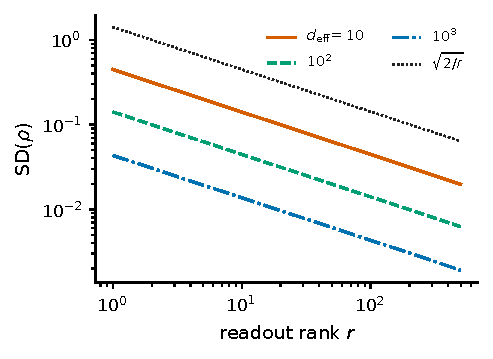
\includegraphics[width=.78\linewidth]{figS2_exact_null_width.pdf}
\caption{Exact random-orientation fluctuation scale for representative effective dimensions. The standard deviation of $\rho$ narrows with increasing readout rank and effective spectral dimension while remaining compatible with a strongly anisotropic covariance when $r d_{\rm eff}$ is large.}
\label{fig:si-null-width}
\end{figure}

\section{Fixed-weight diagonal readout spaces}

For full computational-basis support, the centered outcome space has dimension $N=2^n-1$. Distinct nonidentity diagonal Pauli strings are orthogonal in the uniform Walsh basis, so the cumulative weight-through-$k$ span has dimension
\begin{equation}
 r_{\le k}=\sum_{j=1}^k\binom nj.
\label{eq:si-rank-full}
\end{equation}
For fixed $k$ and large $n$, $r_{\le k}=n^k/k!\,[1+O(n^{-1})]$.

In the half-filled fixed-charge sector, the outcome support contains $\binom{n}{n/2}$ basis strings and the centered score dimension is
\begin{equation}
 N_{\rm hf}=\binom{n}{n/2}-1.
\end{equation}
The identity $\sum_i Z_i=0$ on the half-filled support removes one one-body degree of freedom, giving
\begin{equation}
 r_1=n-1.
\end{equation}
For the cumulative one- and two-body diagonal span, the centered dimension used in the numerical protocol is
\begin{equation}
 r_{\le2}=\binom n2-1.
\end{equation}
These rank identities provide geometric bookkeeping and do not determine the physical orientation of the tangent covariance. Fixed-charge harmonic analysis provides broader mathematical context for low-degree functions on a slice \cite{Filmus2016}.

\begin{figure}[t]
\centering
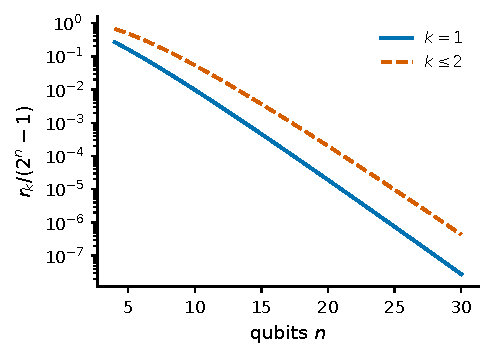
\includegraphics[width=.78\linewidth]{figS4_rank_fraction.pdf}
\caption{Rank fractions for low-weight diagonal readouts under full computational-basis support. Polynomially growing low-weight spaces occupy an exponentially shrinking fraction of the centered record.}
\label{fig:si-rank-fractions}
\end{figure}

\section{Cross-fitting, Ky Fan benchmark, and statistical unit}

For a covariance estimate $\widehat C_{\rm fit}$ obtained from one tangent ensemble, let $Q_r$ contain its leading $r$ eigenvectors and define
\begin{equation}
P_{\rm xfit}=Q_rQ_r^{\mathsf T}.
\end{equation}
Retention is evaluated on an independent tangent ensemble,
\begin{equation}
 R_{\rm xfit}=\frac1{m_{\rm eval}}\sum_{a=1}^{m_{\rm eval}}
\|P_{\rm xfit}u_a^{\rm(eval)}\|_2^2.
\label{eq:si-crossfit}
\end{equation}
This prevents the same tangent samples from both selecting and evaluating the subspace. The frozen operational profile uses 128 alignment tangents and 128 independent evaluation tangents per circuit. The generic Haar-$U(4)$ cells use 16 circuit instances per size and the $U(1)$ cells use 20, with a 10,000-shot finite-shot evaluation model and 8 held-out finite-difference directions. The alignment sample is a separate calibration resource and is not counted as free measurement cost in the fixed-evaluation-budget comparison.

The same-sample Ky Fan quantity
\begin{equation}
R_{\rm KF}=\sum_{j=1}^r\lambda_j(\widehat C)
\end{equation}
is an optimistic spectral upper benchmark rather than the operational estimator \cite{KyFan1949}. The independent resampling unit throughout the statistical analysis is the circuit instance. Confidence intervals resample circuit instances and recompute the relevant aggregate. Frozen profiles, deterministic seeds, shard-level outputs, and paper-facing summaries are archived in the reproducibility repository \cite{AitHaddou2026MeasurementAccessible}.

\section{Finite-shot directional-signal diagnostics}

Let $F_{\rm full}(v)$ denote the classical Fisher scale of direction $v$ before unit normalization. For rank-$r$ projector $P$, define
\begin{equation}
E_{\rm raw}(P)=\mathbb E_v\!\left[F_{\rm full}(v)\,\|Pu_v\|_2^2\right].
\label{eq:si-raw-energy}
\end{equation}
If a scalar readout direction is sampled isotropically inside the retained $r$-dimensional subspace, the mean squared directional signal is
\begin{equation}
\mathbb E[g_{\rm dir}^2]=\frac{E_{\rm raw}(P)}{r}.
\label{eq:si-dir-signal}
\end{equation}
The finite-shot calculation combines this signal with the multinomial covariance of the fixed measurement record. Physical, random-rank, and aligned comparisons keep the circuit, quantum measurement, readout rank, and shot count fixed. These are controlled directional diagnostics, not gradient-variance claims for an arbitrary supervised loss.

\begin{figure}[t]
\centering
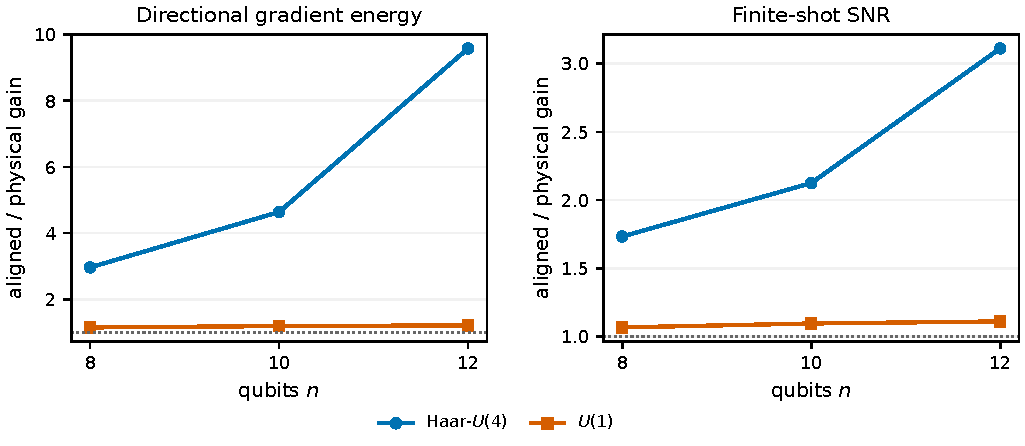
\includegraphics[width=.95\linewidth]{appendix_operational_gains.pdf}
\caption{Additional fixed-rank operational diagnostics. Retention, directional gradient-energy, and finite-shot SNR gains are shown for the physical versus cross-fitted aligned comparison. Generic Haar-$U(4)$ circuits leave substantial room for orientation improvement, whereas the structured $U(1)$ readout is already comparatively aligned.}
\label{fig:si-operational}
\end{figure}

\section{Additional covariance, orientation, and readout-noise diagnostics}

\begin{figure}[t]
\centering
\begin{minipage}{.32\textwidth}\centering
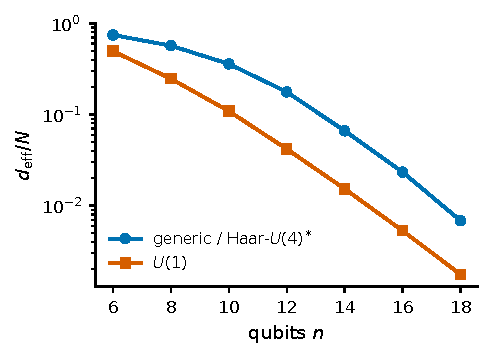
\includegraphics[width=\linewidth]{figS1_deff_fraction.pdf}
\end{minipage}\hfill
\begin{minipage}{.32\textwidth}\centering
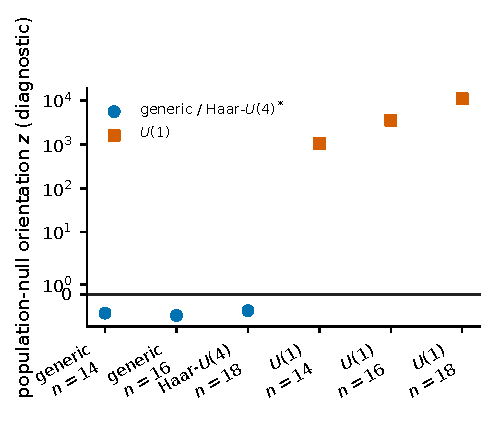
\includegraphics[width=\linewidth]{figS3_orientation_z.pdf}
\end{minipage}\hfill
\begin{minipage}{.32\textwidth}\centering
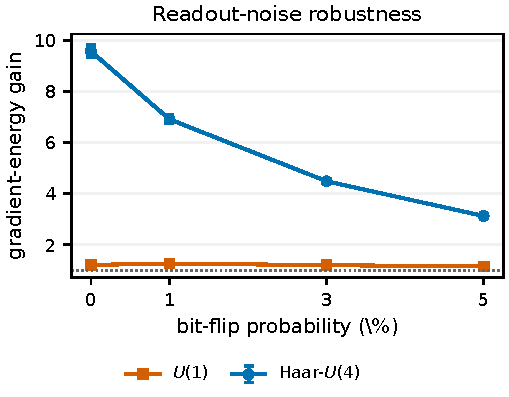
\includegraphics[width=\linewidth]{appendix_noise_robustness.pdf}
\end{minipage}
\caption{Supporting diagnostics. Left: effective spectral fraction $d_{\rm eff}/N$. Center: population-null orientation diagnostic for representative generic/Haar and $U(1)$ points. Right: aligned-to-physical directional gradient-energy gain under readout bit-flip noise. In the noise comparison the aligned subspace is re-estimated after noise is applied; the panel therefore does not establish robustness of one fixed optimized observable.}
\label{fig:si-supporting}
\end{figure}

\section{Finite-size diagnostics for the half-filled $U(1)$ family}

Across $n=8,10,12,14,16,18$, the cross-fitted one-body overlaps are $0.552$, $0.450$, $0.396$, $0.341$, $0.309$, and $0.284$, respectively. At $n=18$,
\begin{equation}
A_1(18)=0.283586\;[0.277044,0.290865],
\end{equation}
and the cumulative weight-through-two overlap is
\begin{equation}
A_{\le2}(18)=0.463538\;[0.457425,0.469591].
\end{equation}
Each size uses 20 independent circuit instances. Two-parameter log-space model comparison over the tested window favors a power form over an exponential form. The fitted exponents are $0.8223\,[0.7694,0.8735]$ for $A_1$ and $0.7041\,[0.6798,0.7281]$ for $A_{\le2}$, with $\Delta\mathrm{AICc}=14.39$ and $12.82$, respectively, in favor of the power model. These results describe finite-size model discrimination only and are not asymptotic bounds or hydrodynamic exponents \cite{AitHaddou2026MeasurementAccessible}.

\begin{figure}[t]
\centering
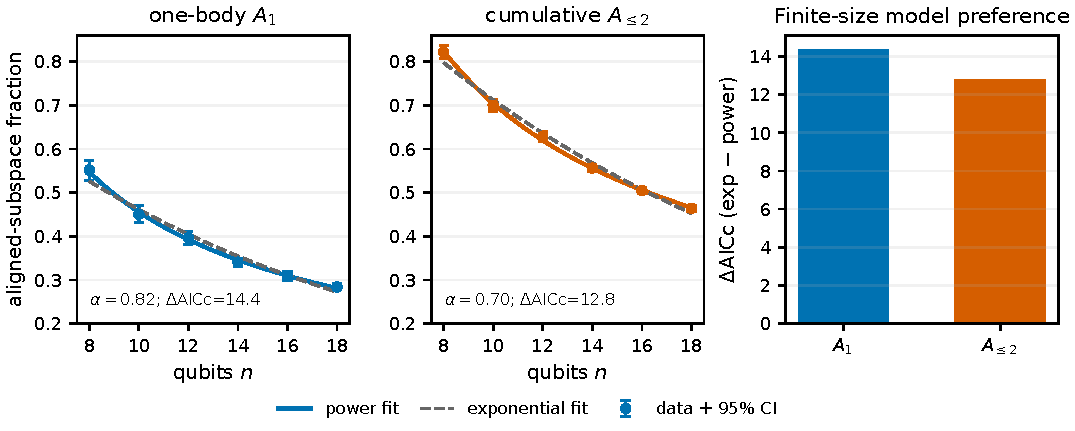
\includegraphics[width=.95\linewidth]{appendix_u1_fit_diagnostics.pdf}
\caption{Finite-size diagnostics for the half-filled $U(1)$ family. The plots compare the measured overlaps with power and exponential fits over $n=8$--$18$ and summarize $\Delta\mathrm{AICc}=\mathrm{AICc}_{\rm exp}-\mathrm{AICc}_{\rm power}$. Positive values favor the power model only within the tested window.}
\label{fig:si-u1-fits}
\end{figure}

\section{Symmetry-breaking sensitivity control}

A separate $n=8$ pilot holds the trainable parameter count fixed while adding a nontrainable perturbation. The unperturbed one-body alignment is
\begin{equation}
A_1=0.517\;[0.486,0.549].
\end{equation}
A symmetry-preserving $R_Z$ perturbation of strength $\epsilon=0.3$ gives
\begin{equation}
A_1=0.481\;[0.454,0.518],
\end{equation}
whereas a symmetry-breaking $R_X$ perturbation at the same strength gives
\begin{equation}
A_1=0.0295\;[0.0248,0.0338].
\end{equation}
The physical one-body retention simultaneously falls from $0.430$ to $0.0325$ in the breaking control \cite{AitHaddou2026MeasurementAccessible}. This pilot establishes sensitivity to charge breaking in the tested setting; it does not identify which microscopic mechanism produces the unperturbed alignment.

\begin{figure}[t]
\centering
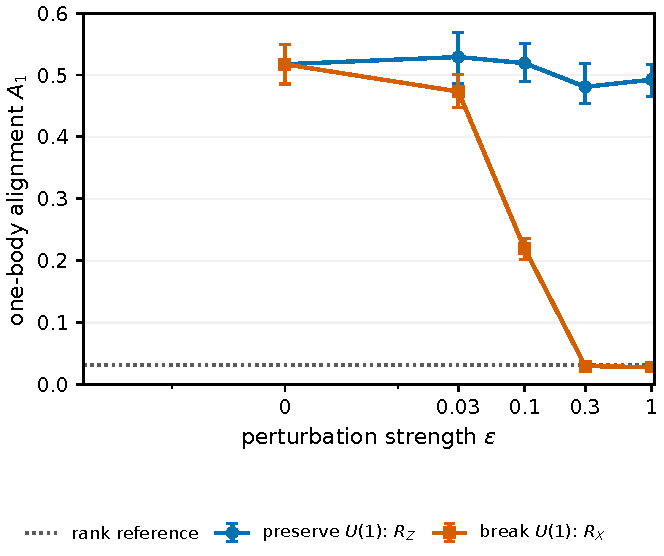
\includegraphics[width=.78\linewidth]{production/fig_symmetry_breaking_control.pdf}
\caption{Symmetry-breaking pilot at $n=8$. Symmetry-preserving $R_Z$ perturbations leave the one-body tangent-subspace overlap comparatively stable, whereas nontrainable $R_X$ perturbations that break charge conservation suppress it toward the full-score-space rank scale. Error bars are 95\% circuit-bootstrap intervals over 10 circuit instances.}
\label{fig:si-symmetry-breaking}
\end{figure}

\section{Circuit conventions and reproducibility}

The numerical campaign uses RY--RZ--CZ, SU2--CNOT, SU2--CZ ring, SU2--CZ random-matching, Haar-$U(4)$ brickwork, and half-filled $U(1)$ RZ--XY circuit families. The PennyLane drawings below are schematics; parameter values are suppressed and representative layers are shown for legibility. Simulations use the exact gate constructors, depth conventions, deterministic seeds, and frozen experiment profiles archived in the repository \cite{Bergholm2018,AitHaddou2026MeasurementAccessible}.

\begin{figure}[t]
\centering
\begin{minipage}{.32\textwidth}\centering
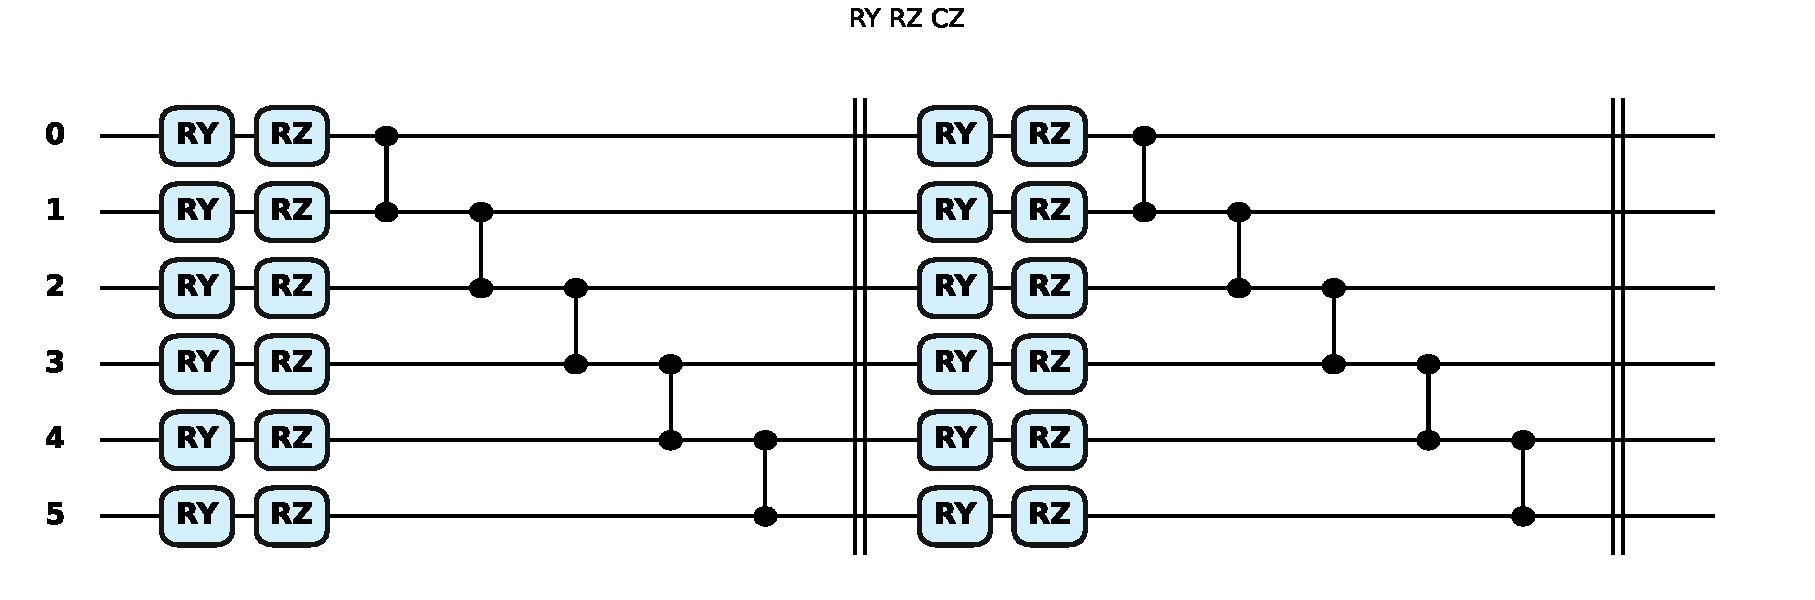
\includegraphics[width=\linewidth]{generated_circuits/circuit_ry_rz_cz.pdf}\\[-1mm]{\scriptsize RY--RZ--CZ}
\end{minipage}\hfill
\begin{minipage}{.32\textwidth}\centering
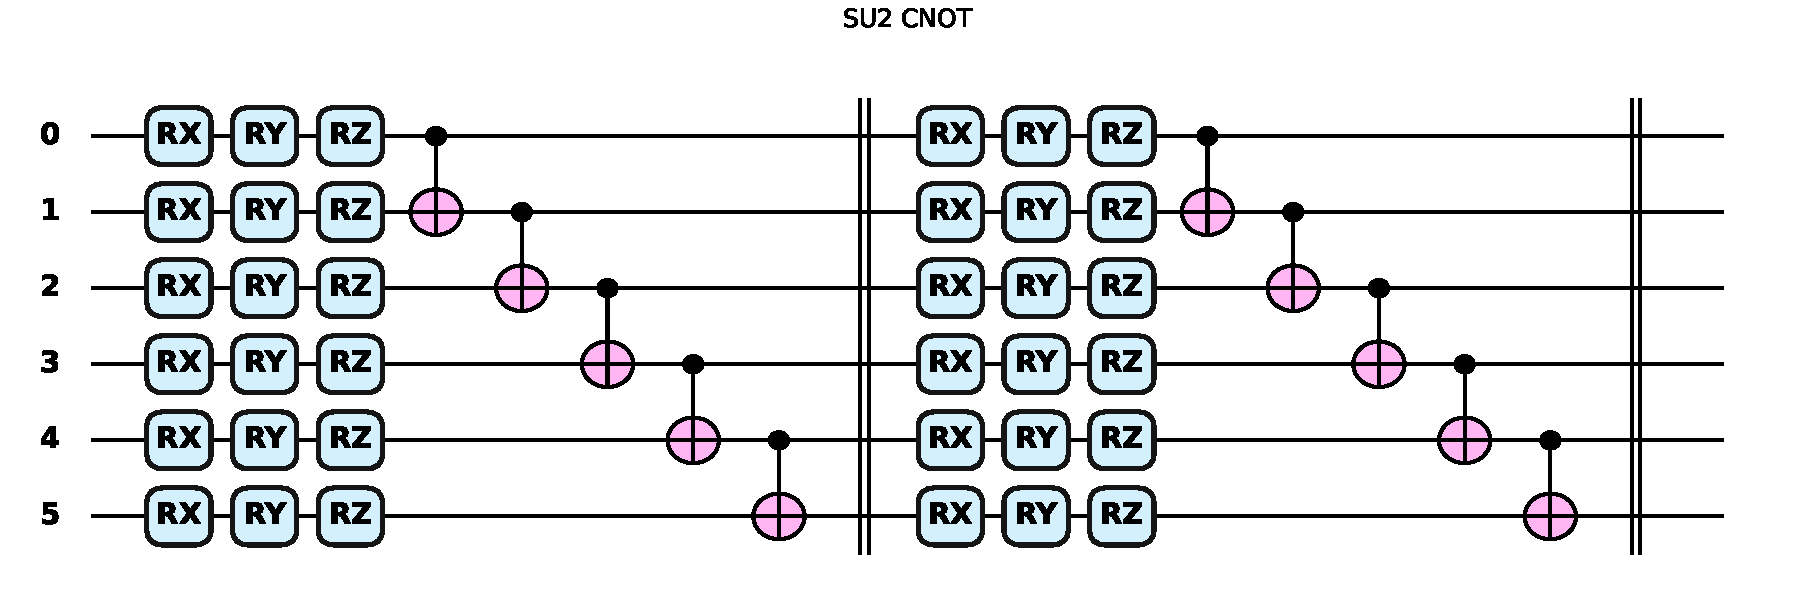
\includegraphics[width=\linewidth]{generated_circuits/circuit_su2_cnot.pdf}\\[-1mm]{\scriptsize SU2--CNOT}
\end{minipage}\hfill
\begin{minipage}{.32\textwidth}\centering
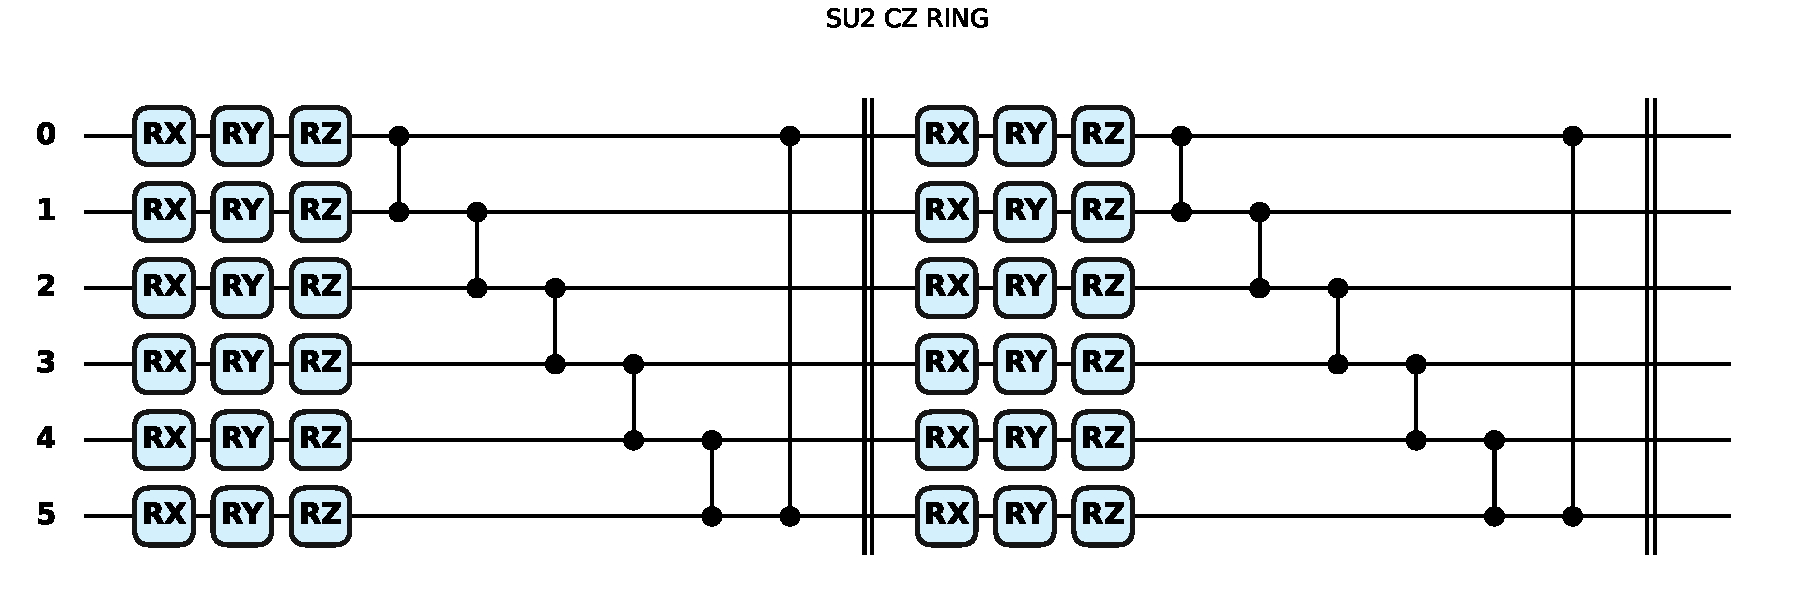
\includegraphics[width=\linewidth]{generated_circuits/circuit_su2_cz_ring.pdf}\\[-1mm]{\scriptsize SU2--CZ ring}
\end{minipage}

\vspace{2mm}
\begin{minipage}{.32\textwidth}\centering
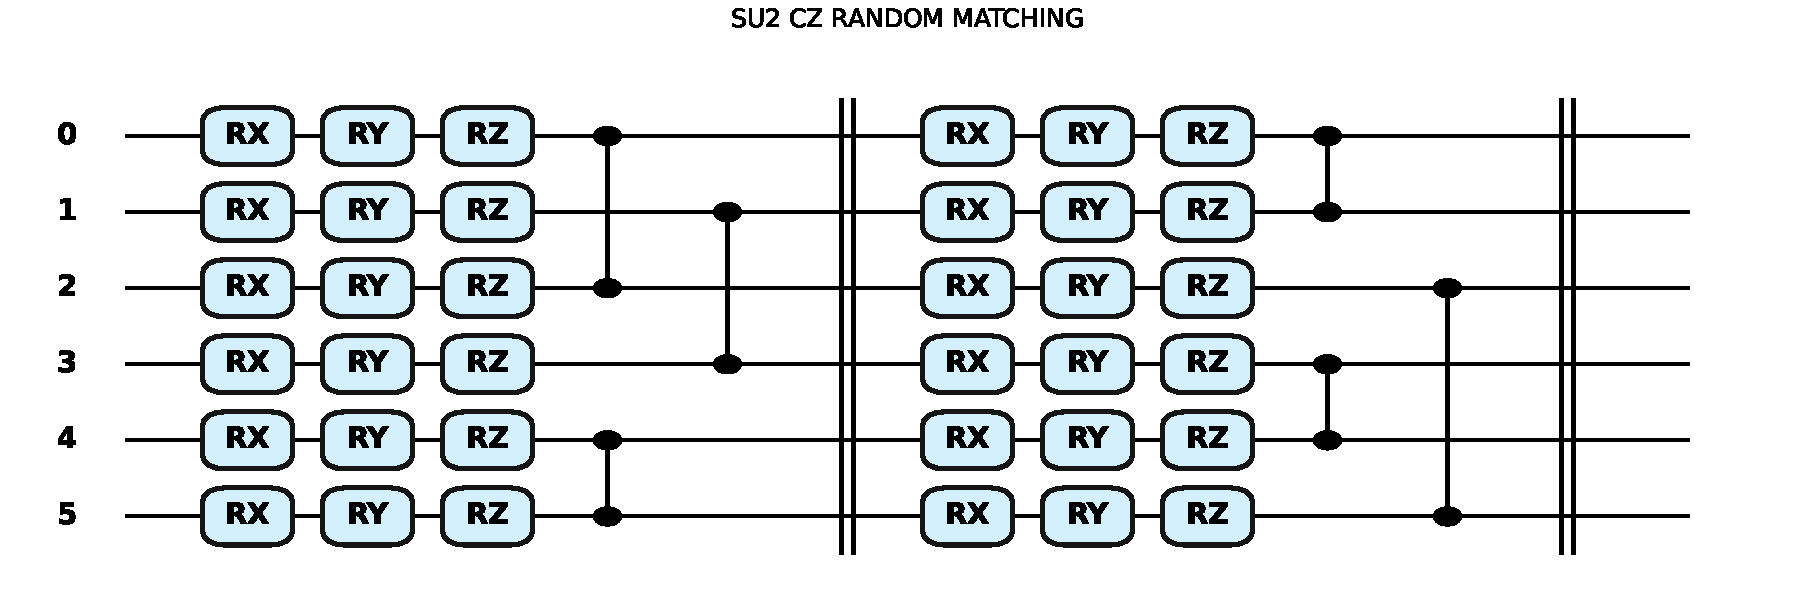
\includegraphics[width=\linewidth]{generated_circuits/circuit_su2_cz_random_matching.pdf}\\[-1mm]{\scriptsize SU2--CZ random matching}
\end{minipage}\hfill
\begin{minipage}{.32\textwidth}\centering
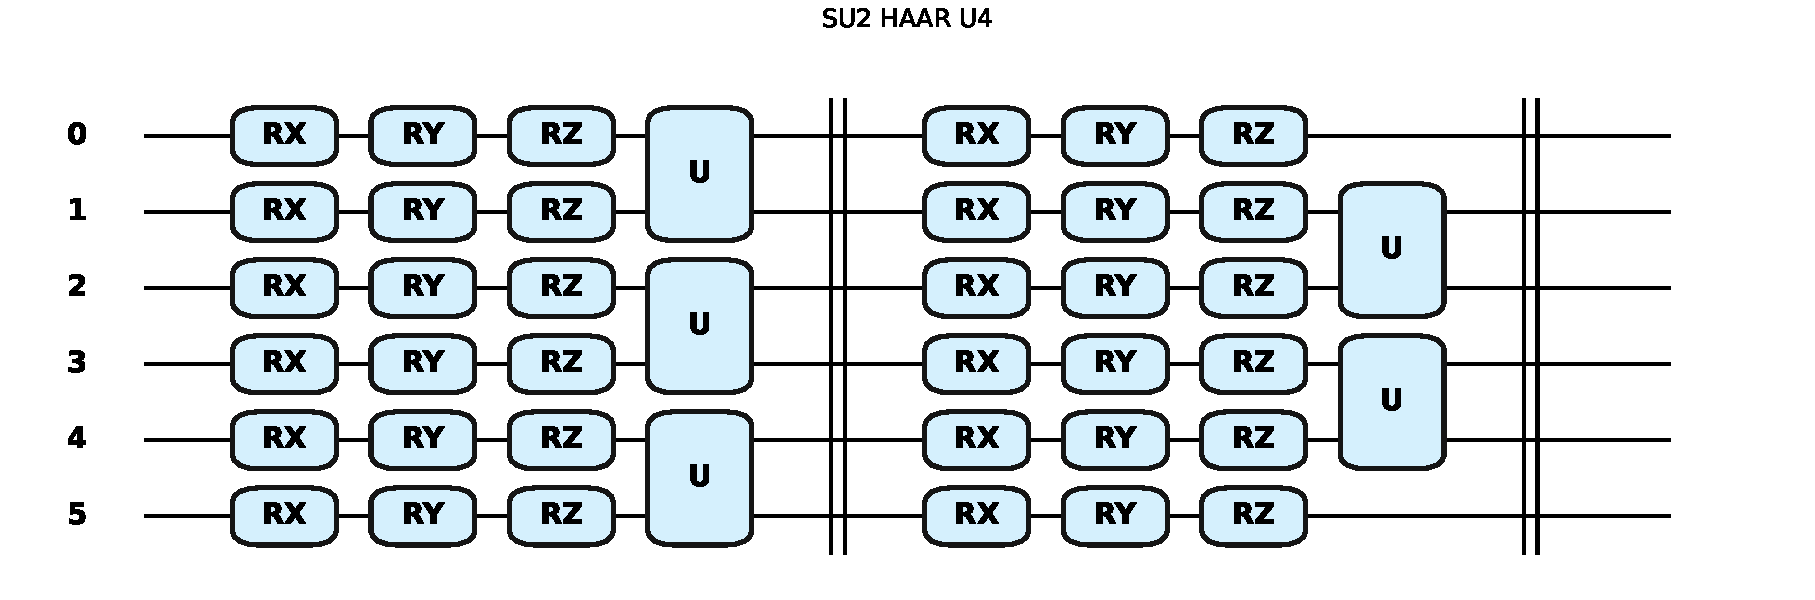
\includegraphics[width=\linewidth]{generated_circuits/circuit_su2_haar_u4.pdf}\\[-1mm]{\scriptsize Haar-$U(4)$ brickwork}
\end{minipage}\hfill
\begin{minipage}{.32\textwidth}\centering
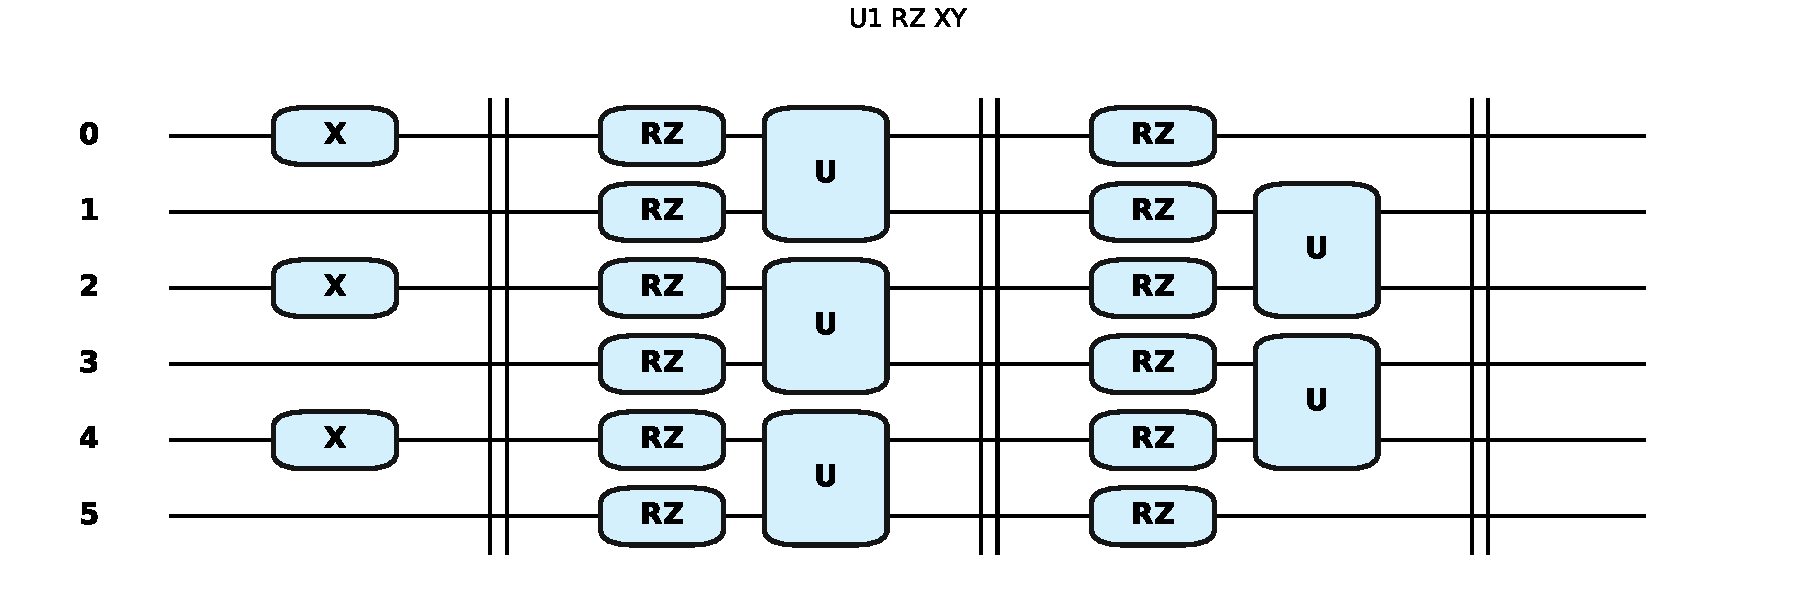
\includegraphics[width=\linewidth]{generated_circuits/circuit_u1_rz_xy.pdf}\\[-1mm]{\scriptsize half-filled $U(1)$ RZ--XY}
\end{minipage}
\caption{Circuit schematics corresponding to the families used in the numerical campaign.}
\label{fig:si-circuits}
\end{figure}

\section{Data and code provenance}

The reproducibility repository contains frozen experiment profiles, source code, deterministic seeds, aggregate tables, shard-level outputs, analysis scripts, and the paper-facing summaries used for the numerical values in the main article and this Supporting Information \cite{AitHaddou2026MeasurementAccessible}. The AQT release candidate additionally includes `.zenodo.json` and `CITATION.cff` metadata for archival of the frozen repository release.

\begin{thebibliography}{99}

\bibitem{BraunsteinCaves1994}
S. L. Braunstein and C. M. Caves,
``Statistical Distance and the Geometry of Quantum States,''
Physical Review Letters \textbf{72}, 3439 (1994), doi:10.1103/PhysRevLett.72.3439.

\bibitem{Stokes2020}
J. Stokes, J. Izaac, N. Killoran, and G. Carleo,
``Quantum Natural Gradient,''
Quantum \textbf{4}, 269 (2020), doi:10.22331/q-2020-05-25-269.

\bibitem{Haug2021}
T. Haug, K. Bharti, and M. S. Kim,
``Capacity and Quantum Geometry of Parametrized Quantum Circuits,''
PRX Quantum \textbf{2}, 040309 (2021), doi:10.1103/PRXQuantum.2.040309.

\bibitem{HottaOzawa2004}
M. Hotta and M. Ozawa,
``Quantum Estimation by Local Observables,''
Physical Review A \textbf{70}, 022327 (2004), doi:10.1103/PhysRevA.70.022327.

\bibitem{LuLuoOh2012}
X.-M. Lu, S. Luo, and C. H. Oh,
``Hierarchy of Measurement-Induced Fisher Information for Composite States,''
Physical Review A \textbf{86}, 022342 (2012), doi:10.1103/PhysRevA.86.022342.

\bibitem{GrossRieser2026}
M. Gross and H.-M. Rieser,
``Theory and Interpretability of Quantum Extreme Learning Machines: A Pauli-Transfer Matrix Approach,''
arXiv:2602.18377 [quant-ph] (2026).

\bibitem{AitHaddou2026IsotropicRankLaws}
M. Ait Haddou,
``Readout-Rank Laws for Isotropic Quantum Tangents,''
arXiv:2608.07628 [quant-ph] (2026).

\bibitem{CollinsMatsumoto2017}
B. Collins and S. Matsumoto,
``Weingarten Calculus via Orthogonality Relations: New Applications,''
ALEA Latin American Journal of Probability and Mathematical Statistics \textbf{14}, 631 (2017), doi:10.30757/ALEA.v14-31.

\bibitem{Bendokat2024}
T. Bendokat, R. Zimmermann, and P.-A. Absil,
``A Grassmann Manifold Handbook: Basic Geometry and Computational Aspects,''
Advances in Computational Mathematics \textbf{50}, 6 (2024), doi:10.1007/s10444-023-10090-8.

\bibitem{KyFan1949}
K. Fan,
``On a Theorem of Weyl Concerning Eigenvalues of Linear Transformations I,''
Proceedings of the National Academy of Sciences of the United States of America \textbf{35}, 652 (1949), doi:10.1073/pnas.35.11.652.

\bibitem{Bergholm2018}
V. Bergholm, J. Izaac, M. Schuld, et al.,
``PennyLane: Automatic Differentiation of Hybrid Quantum-Classical Computations,''
arXiv:1811.04968 (2018).

\bibitem{AitHaddou2026MeasurementAccessible}
M. Ait Haddou,
``Spectral Geometry of Accessible Quantum Tangents: Reproducibility Repository,''
GitHub repository (2026),
\url{https://github.com/AHDMarwan/Spectral-Geometry-of-Accessible-Quantum-Tangents-Beyond-Isotropic-Readout-Rank-Laws}.

\bibitem{Efron1979}
B. Efron,
``Bootstrap Methods: Another Look at the Jackknife,''
The Annals of Statistics \textbf{7}, 1 (1979), doi:10.1214/aos/1176344552.

\bibitem{LuSha2025}
J. Lu and K. Sha,
``Quantum Fisher Information Matrix via Its Classical Counterpart from Random Measurements,''
arXiv:2509.08196 (2025).

\bibitem{Monbroussou2025}
L. Monbroussou, E. Z. Mamon, J. Landman, et al.,
``Trainability and Expressivity of Hamming-Weight Preserving Quantum Circuits for Machine Learning,''
Quantum \textbf{9}, 1745 (2025), doi:10.22331/q-2025-05-15-1745.

\bibitem{Fontana2024}
E. Fontana, D. Herman, S. Chakrabarti, et al.,
``Characterizing Barren Plateaus in Quantum Ans\"atze with the Adjoint Representation,''
Nature Communications \textbf{15}, 7171 (2024), doi:10.1038/s41467-024-49910-w.

\bibitem{Ragone2024}
M. Ragone, B. N. Bakalov, F. Sauvage, et al.,
``A Lie Algebraic Theory of Barren Plateaus for Deep Parameterized Quantum Circuits,''
Nature Communications \textbf{15}, 7172 (2024), doi:10.1038/s41467-024-49909-3.

\bibitem{Filmus2016}
Y. Filmus,
``An Orthogonal Basis for Functions over a Slice of the Boolean Hypercube,''
The Electronic Journal of Combinatorics \textbf{23}(1), P1.23 (2016), doi:10.37236/4567.

\bibitem{Khemani2018}
V. Khemani, A. Vishwanath, and D. A. Huse,
``Operator Spreading and the Emergence of Dissipative Hydrodynamics under Unitary Evolution with Conservation Laws,''
Physical Review X \textbf{8}, 031057 (2018), doi:10.1103/PhysRevX.8.031057.

\bibitem{Rakovszky2018}
T. Rakovszky, F. Pollmann, and C. W. von Keyserlingk,
``Diffusive Hydrodynamics of Out-of-Time-Ordered Correlators with Charge Conservation,''
Physical Review X \textbf{8}, 031058 (2018), doi:10.1103/PhysRevX.8.031058.

\end{thebibliography}


\end{document}
